\documentclass{thesisclass}

%% Bibstyle %%
\usepackage[numbers]{natbib}
\usepackage{float}
\usepackage{multirow}
\usepackage{listings}
\usepackage{placeins}
\usepackage{graphicx}
% My OWN PACKAGES %
\usepackage[T1]{fontenc}
\usepackage[ngerman]{babel}
\usepackage{amsfonts}
\def\UrlBreaks{\do\/\do-}
%Predefined paths%
\graphicspath{ {images/} }
%My own predefined paths%
%OWN STUFF%
%% Glossar %%
\usepackage[toc,nonumberlist]{glossaries}
\makeglossaries

% Glossary


\newglossaryentry{IA}{
	name=IA,
	description=Intelligenter (persönlicher) Assistent
}

\newglossaryentry{KI}{
	name=KI,
	description = Jegliches Programm\, das es einer Maschine erm\"oglicht auf ihre Umwelt zu reagieren.
}

\newglossaryentry{MaschinellesLernen}{
	name = ML,
	description = Maschinelles Lernen\, künstliche generierung von Wissen aus Erfahrung.
}

\newglossaryentry{ANN}{
	name = ANN,
	description = Artificial Neural Network\, ein Künstliches Neuronales Netz.
}

\newglossaryentry{FFN}{
	name = FFN,
	description = Feed Forward Network\, ein Künstliches Neuronales Netz dessen Neuronen einen Azyklischen Graph bilden.
}

\newglossaryentry{FCNN}{
	name = Fully connected Neural Network,
	description = ein Neuronales Netz\, in dem jede Lage mit der nächsten verbunden ist.
}

\newglossaryentry{RNN}{
	name = RNN,
	description = Recurrent Neural Network\, ein Neuronales Netz\, das im gegenzug zu Feed Forward Netzten es erlaubt Signale an vorangehende Schichten zurückzugeben.
}

\newglossaryentry{test}{
name = testosterone,
description = itworks
}

\newglossaryentry{MT}{
name = MT,
description = Machine Translation\, eine automatische Übersetzung von geschriebener oder gesprochener Sprache in eine andere Sprache bzw. Form.
} 

\newglossaryentry{NMT}{
name = NMT,
description = Neural machine translation\, automatische Übersetzung von geschriebener oder gesprochener Sprache in eine andere Sprache bzw. Form mithilfe von Künstlichen Neuronalen Netzen (ANN).
}

\newglossaryentry{NLP}{
name = NLP,
description = natural language programming\, Programmieren in natürlicher Sprache\, z.B Deutsch oder Englisch.
}

\newglossaryentry{Backpropagation}{
	name = Backpropagation,
	description = Ein Werkzeug das es ANN ermöglicht zu trainieren. Weights und Biases werden geupdated.
}

\newglossaryentry{Tensorflow}{
	name = Tensorflow,
	description = Ein Open Source Framework für ANN von Google.
}

\newglossaryentry{Ausreisser}{
	name = Ausreißer,
	description = Ein Funktionswert\, der um ein vielfaches von seinem zeitlich vorgehenden Wert abweicht.
}

\newglossaryentry{Turingtest}{
	name = Turingtest,
	description = ein von Alan Turing entwickelter Test\, ob eine Maschine ein dem Menschen gleichwertiges Denkvermögen hat
	}

\lstset{language=Java,
   basicstyle=\small,
   keywordstyle=\color{blue!80!black!100},
   identifierstyle=,
   commentstyle=\color{green!50!black!100},
   stringstyle=\ttfamily,
   breaklines=true,
   %numbers=left,
   numberstyle=\small,
   %frame=single,
   backgroundcolor=\color{blue!3}
} 
\renewcommand*{\lstlistingname}{Quelltextausschnitt}


% Based on thesisclass.cls of Timo Rohrberg, 2009
% ----------------------------------------------------------------
% Thesis - Main document
% ----------------------------------------------------------------

%% ---------------------------------
%% | Information about the thesis  |
%% ---------------------------------

\newcommand{\myname}{Philipp Weinmann}
\newcommand{\mytitle}{Maschinelles Lernen im Kontext der Programmierung in natürlicher Sprache}
\newcommand{\myinstitute}{Institut f\"ur Programmstrukturen\\
											und Datenorganisation (IPD)}
											
\newcommand{\advisor}{Dipl. Inform. Alexander Wachtel}

%\newcommand{\timestart}{Startdatum}
%\newcommand{\timeend}{Enddatum}
\newcommand{\submissiontime}{14/01/19}


%% -------------------------------
%% |  Information for PDF file   |
%% -------------------------------
\hypersetup{
 pdfauthor={\myname},
 pdftitle={\mytitle},
 pdfsubject={Not set},
 pdfkeywords={Not set}
}

%%%%%%%%%%%%%%%%%%%%%%%%%%%%%%%%%
%% Here, main documents begins %%
%%%%%%%%%%%%%%%%%%%%%%%%%%%%%%%%%
\begin{document}

% Describe separation hints here: %
%% --------------------------------
%% | Settings for word separation |
%% --------------------------------
% Help for separation:
% In german package the following hints are additionally available:
% "- = Additional separation
% "| = Suppress ligation and possible separation (e.g. Schaf"|fell)
% "~ = Hyphenation without separation (e.g. bergauf und "~ab)
% "= = Hyphenation with separation before and after
% "" = Separation without a hyphenation (e.g. und/""oder)

\hyphenation{
Sprach-ein-ga-ben
}

\selectlanguage{ngerman}
\floatname{algorithm}{Algorithmus}

\frontmatter
\pagenumbering{roman}
%% titlepage.tex
%%

% coordinates for the bg shape on the titlepage
\newcommand{\diameter}{20}
\newcommand{\xone}{-15}
\newcommand{\xtwo}{160}
\newcommand{\yone}{15}
\newcommand{\ytwo}{-253}

\begin{titlepage}
% bg shape
\begin{tikzpicture}[overlay]
\draw[color=gray]  
 		 (\xone mm, \yone mm)
  -- (\xtwo mm, \yone mm)
 arc (90:0:\diameter pt) 
  -- (\xtwo mm + \diameter pt , \ytwo mm) 
	-- (\xone mm + \diameter pt , \ytwo mm)
 arc (270:180:\diameter pt)
	-- (\xone mm, \yone mm);
\end{tikzpicture}
	\begin{textblock}{10}[0,0](4,2.5)
		
\includegraphics[width=.3\textwidth]{logos/KITLogo_RGB.pdf}
	\end{textblock}
	\changefont{phv}{m}{n}	% helvetica	
	\vspace*{3.5cm}
	\begin{center}
		\Huge{\mytitle}
		\vspace*{2cm}\\
		\Large{
			\iflanguage{english}{Seminar Paper of}			
												  {Seminararbeit \\von} 
		}\\
		\vspace*{1cm}
		\huge{\myname}\\
		\vspace*{1cm}
		\Large{
			\iflanguage{english}{At the Department of Informatics}			
													{An der Fakult\"at f\"ur Informatik}
			\\
			\myinstitute
		}
	\end{center}
	\vspace*{1cm}
\Large{
\begin{center}
\begin{tabular}[ht]{l c l}
  % Gutachter sind die Professoren, die die Arbeit bewerten. 
%  \iflanguage{english}{Reviewer}{Erstgutachter}: & \hfill  & \reviewerone\\
 % \iflanguage{english}{Second reviewer}{Zweitgutachter}: & \hfill  & \reviewertwo\\
  \iflanguage{english}{Advisor}{Betreuer}: & \hfill  & \advisor\\
 % \iflanguage{english}{Second advisor}{Zweiter Betreuer}: & \hfill  & \advisortwo\\
  % Der zweite betreuende Mitarbeiter kann weggelassen werden. 
\end{tabular}
\end{center}
}


%\vspace{2cm}
%\begin{center}
%\large{\iflanguage{english}{Duration:}{Bearbeitungszeit}: \timestart \hspace*{0.25cm} -- \hspace*{0.25cm} \timeend}
%\end{center}


\begin{textblock}{10}[0,0](4,16.8)
\tiny{ 
	\iflanguage{english}
		{KIT -- University of the State of Baden-Wuerttemberg and National Research Center of the Helmholtz Association}
		{KIT -- Universit\"at des Landes Baden-W\"urttemberg und nationales Forschungszentrum in der Helmholtz-Gemeinschaft}
}
\end{textblock}

\begin{textblock}{10}[0,0](14,16.75)
\large{
	\textbf{www.kit.edu} 
}
\end{textblock}

\end{titlepage}

\blankpage
\vspace*{36\baselineskip}
\hbox to \textwidth{\hrulefill}
\par
\iflanguage{english}{I declare that I have developed and written the enclosed thesis completely by myself, and have not used sources or means without declaration in the text.}{Ich versichere wahrheitsgem\"a\ss, die Arbeit selbstst\"andig angefertigt, alle benutzten Hilfsmittel vollst\"andig und genau angegeben und alles kenntlich gemacht zu haben, was aus Arbeiten anderer unver\"andert oder mit Ab\"anderungen entnommen wurde.}

\iflanguage{english}{I followed the rules for securing a good scientific pracise of the Karlsruhe Institute of Technology (Regeln zur Sicherung guter wissenschaftlicher Praxis im Karlsruher Institut f\"ur Technologie (KIT)).}{Die Regeln zur Sicherung guter wissenschaftlicher Praxis im Karlsruher Institut f\"ur Technologie (KIT) habe ich befolgt.}

\textbf{Karlsruhe, \submissiontime{}}
\vspace{1.5cm}

\dotfill\hspace*{8.0cm}\\
\hspace*{2cm}(\textbf{\myname{}}) %center name with hspace

\thispagestyle{empty}

\blankpage

%inspirational quote%
%vspace centers the quote horizontally%
%\vspace*{\fill}
%\begin{figure}[h]
% \center
%  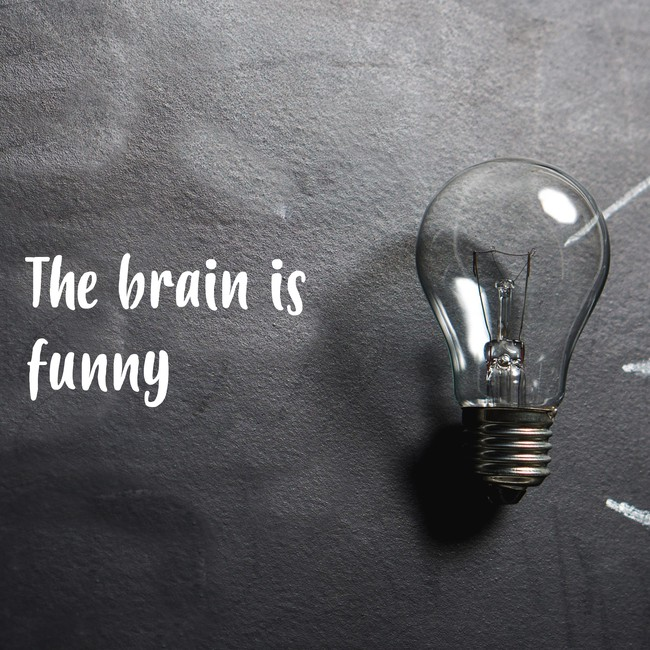
\includegraphics[width=250px]{images/inspirobotQuote.jpg}
%  \caption{Ein Zitat, das von einer Künstlichen Intelligenz (\gls{KI}) generiert wurde. \textit{Die Resultate sind noch nicht zufriedenstellend} \cite{inspirobot}}
%  \label{fig:Inspirational quote by AI}
%\end{figure}
%\vspace*{\fill}\clearpage

%% -------------------
%% |   Directories   |
%% -------------------
\tableofcontents
\cleardoublepage

%\listoffigures
%
%\listoftables
%\cleardoublepage



%% -----------------
%% |   Main part   |
%% -----------------
\mainmatter
\pagenumbering{arabic}

%Abstract%
\chapter*{Abstract}
%[TODO] Ein Abstract ist eine prägnante Inhaltsangabe, ein Abriss ohne Interpretation %und Wertung einer wissenschaftlichen Arbeit.
Der Forschungsbereich Programmieren in Natürlicher Sprache findet erst seit kurzem größeres Interesse. Dies geschieht in einer Zeit, in der das Maschinelle Lernen an Bedeutung gewinnt. Es ist daher interessant zu betrachten, welche Anwendungsmöglichkeiten Maschinelles Lernen in diesem Bereich der Informatik bietet. In dieser Arbeit werden wir betrachten, was unter dem Begriff Maschinelles Lernen zu verstehen ist und gehen auf Künstliche Neuronalen Netze (\gls{ANN}s), die Teil von Maschinellem Lernen sind, genauer ein. Des Weiteren werden wir die Vorteile der Anwendung von \gls{ANN}s für die maschinelle Übersetzung betrachten und bewerten.
\newpage
\let\cleardoublepage\relax \chapter{Einleitung}
\begin{figure}[H]
  \center
  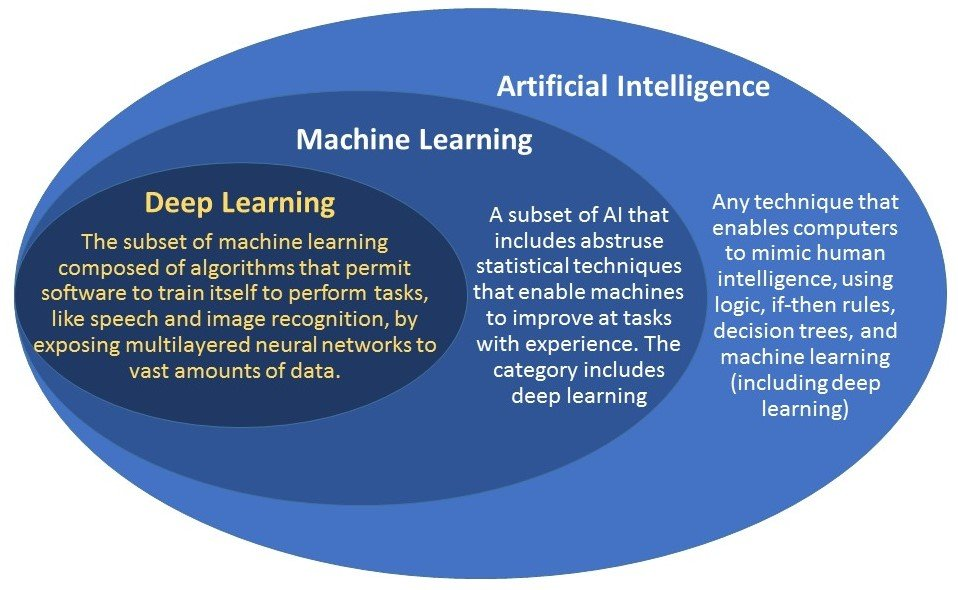
\includegraphics[width=\textwidth]{images/machineLearningInAI.jpg}
  \caption{Veranschaulichung, wie Maschinelles Lernen einzuordnen ist. \cite{machineLearning1}}
  \label{fig:Veranschaulichung, wie Maschinelles Lernen einzuordnen ist.}
\end{figure}

Maschinelles Lernen (\gls{MaschinellesLernen}) ist, wie in Abbildung 1.1 beschrieben, ein Teilbereich der K\"unstlichen Intelligenz (\gls{KI}). Es ist ein Oberbegriff für die künstliche Generierung von Wissen aus Erfahrung \cite{eter_2018}. Weil es oft schwierig ist, bei einer Entscheidung zu erkennen, welche Option das beste Ergebnis liefert, versuchen moderne Programme dies maschinell zu lösen. Dank statistischer Auswertungen k\"onnen Algorithmen entstehen, die mit einer gewissen Wahrscheinlichkeit korrekte Ergebnisse liefern, ohne das der Programmierer sich Gedanken machen muss, wie der Algorithmus im Detail aufgebaut ist.\newline

\section{Anwendungen im Bereich der Informatik}
	In jedem Gebiet, in dem große Mengen an Daten zur Verf\"ugung stehen bzw. generiert werden können, ist \gls{MaschinellesLernen} theoretisch anwendbar.\cite{kour_2018}.
Obwohl die Theorie hinter dieser Art der Datenauswertung seit langem bekannt ist, so finden m\"achtigere Algorithmen, die z.B. auf Künstlichen Neuronalen Netzen (\gls{ANN}s) basieren, erst seit kurzem verbreitete Anwendung. Dies wird allgemein auf die verbesserte Rechenleistung modernen Computer zurückgeführt. \cite{DBLP:journals/corr/abs-1803-08971} \newline
	\newline Anwendungsbereiche sind zum Beispiel:
\begin{itemize}
	\item Gesichtserkennung
	\item Spamerkennung (Email)
	\item Umwandlung von gesprochener Sprache zu Text
	\item Handschrifterkennung
	\item Autonomes Fahren
	\item Automatische Medikamentenentwicklung
	\item Maschinelle Übersetzungen
\end{itemize}

In dieser Ausarbeitung werden wir uns insbesondere für Künstliche Neuronale Netze (\gls{ANN}s) sowie deren Anwendung für maschinelle Übersetzungen interessieren.

\section{Maschinelles Lernen: Ein erstes Beispiel}
	Hören sie sich dieses Beispiel an: \hyperlink{https://www.audioblocks.com/stock-audio/playground-children-playing.html}{https://www.audioblocks.com/stock-audio/playground-children-playing.html}\newline
	Sie erkennen sofort, dass es sich um spielende Kinder handelt. Unser Gehirn schafft es mit extremer Genauigkeit komplexe Geräusche zu erkennen und zu analysieren. Auch wenn wir nicht ausmachen können, was jedes einzelne Kind ruft, so wissen wir instinktiv dass es sich um Kinder handelt. Schauen wir uns einmal die Wellenfunktion eines Abschnittes dieses Audiofiles an:
\begin{figure}[H]
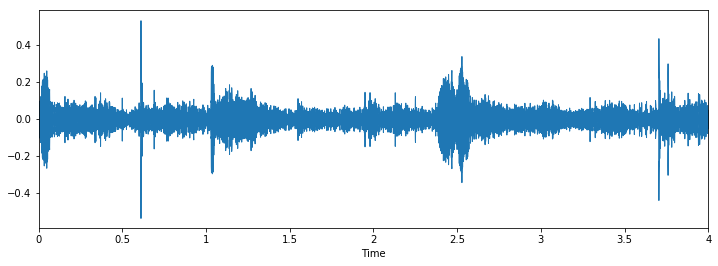
\includegraphics[width=\textwidth]{images/KidsPlaying.png}
  \caption{Audiofile spielender Kinder. Luftdruck/Umgebungsdruck in Funktion der Zeit  (Sekunden). \cite{shaikh_faizan_2017}}
  \label{fig:Audiofile Spielende Kinder}
\end{figure}

Betrachten wir Wellenfunktion eines Presslufthammers, bekommen wir eine sehr unterschiedliche Wellenfunktion:
\begin{figure}[H]
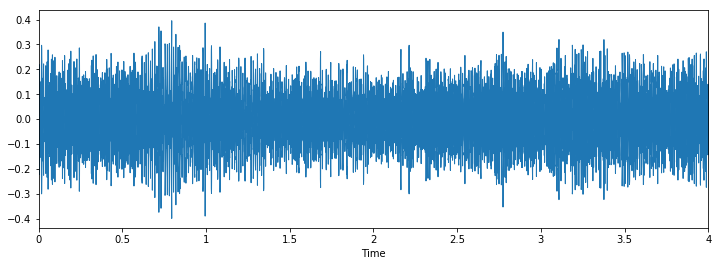
\includegraphics[width=\textwidth]{images/jackhammer.png}
  \caption{Audiofile eines Presslufthammers. Luftdruck/Umgebungsdruck in Funktion der Zeit  (Sekunden). \cite{shaikh_faizan_2017}}
  \label{fig:Audiofile pressluftHammer}
\end{figure}

Wir können einige klare Unterschiede ausmachen. Falls wir nun ein Programm schreiben wollen, das erkennt ob ein Audiofile spielende Kinder oder das Geräusch eines Presslufthammers enthält, so können wir anhand der Wellenfunktion dieser Geräusche einige Lösungsansätze folgern. Wir bemerken zum Beispiel, dass es bei kreischenden Kindern deutlich mehr \gls{Ausreisser} gibt als bei dem Geräusch eines Presslufthammers. Wir könnten also ein Programm schreiben, das ein Audiofile nach der Anzahl an Ausreißern pro Sekunde (\textbf{APS}) erkennt, d.h. klassifiziert.

\begin{lstlisting}
String classify(int[] audiofile) {
   	float APS = getAPS(audiofile); 	// AusreisserProSekunde
	if (APS > (spielkinderDurchschnittsAPS + pressluftHammerDurchschnittsAPS) / 2)){
		return "SpielendeKinder";
	} else {
		return "PressluftHammer";
	}
}
\end{lstlisting}

Um diesen Code ausführen zu können muss bekannt sein, welchen Wert die Ausreißer pro Sekunde (\textbf{APS}) von spielenden Kindern bzw. von Presslufthämmern im Durchschnitt annehmen. Um dies Abzuschätzen, ist ein großer Datensatz an Audiodateien, bei denen bekannt ist um welche Geräusche es sich handelt, nötig. Falls dieser vorhanden sind, kann folgendes Programm geschrieben werden, welches den Durchschnittswert der Ausreißer pro Sekunde  (\textbf{APS}) für die jeweilige Kategorie ermittelt:
\clearpage

\begin{lstlisting}
float mittelwertAPS = (spielkinderDurchschnittsAPS + pressluftHammerDurchschnittsAPS) / 2);
    String classify(int[] audiofile, String category) {
        	float APS = getAPS(audiofile);
			if (APS > mittelwertAPS){
				updateAPS(APS, category);		
				return "SpielendeKinder";
			} else {
				updateAPS(APS, category);
				return "PressluftHammer";
			}
    }   
void updateAPS(int APS, String category) {
	if(category.equals(spielendeKinder)) {
		spielendeKinderAPSList.add(APS);
	} else {
		pressluftHammerAPSList.add(APS);
	}
}
\end{lstlisting}

Dieses zweite Programm ermittelt noch immer, welcher Kategorie die Audiofiles angehören. Daher kann es, falls bekannt ist um welche der beiden Kategorien es sich handelt weiterverwendet werden. Die Ausreißer pro Sekunde (\textbf{APS}) werden damit mit jedem neuen vorklassifizierten Audiofile (\textit{labeled data}) präziser und das Programm lernt mit der Zeit. Dies ist ein Beispiel sehr rudimentärem Maschinellem Lernen.\newline
Es gibt mächtigere Programme, in denen der Algorithmus nicht nur den Wert einer Variablen erkennt, sondern auch die Kriterien zur Unterscheidung zwischen Kategorien oder sogar Kategorien selber ermittelt.

\section{Aufkommen von Maschinellem Lernen}

Maschinelles Lernen generell und insbesondere Neuronale Netze erfreuen sich seit einigen Jahren großer Aufmerksamkeit. Anfangs wurden erst statistische Analysemethoden entdeckt und verbessert \cite{bayes1763essay}\cite{legendre1805nouvelles}\cite{markov2006example}. %Dort analysiert Markov ein Gedicht und bemerkt, das man Wahrscheinlichkeiten formulieren kann, welche Eigenschaften weitere Teile vom Text haben ohne das man die Gesamtheit des Gedichtes in Betracht ziehen muss. \newline
Ab der zweiten Hälfte des 20. Jahrhunderts, mit der Entwicklung der ersten Computern, werden mehrere Pionierarbeiten über das Maschinelle Lernen publiziert. 1950 formuliert Alan Turing die Turing Learning Machine \cite{machinery1950computing}, ein Jahr später entwickeln und bauen zwei Wissenschaftler das erste neuronale Netz \cite{snarc}. 1957 entwickelt Frank Rosenblatt den "perceptron" \cite{rosenblatt1958perceptron}, ein erstes Modell eines vollständig verbundenen neuronalen Netzes (\gls{FCNN}), siehe Abbildung 1.4.

\begin{figure}[H]
  \center
  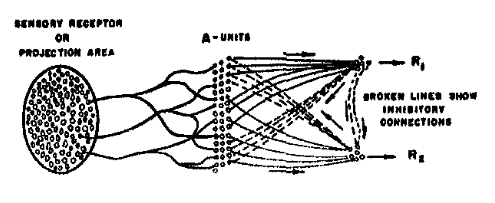
\includegraphics[width=\textwidth]{images/perceptron.png}
  \caption{Zeichnung eines Perceptrons in der ursprünglichen Arbeit. \cite{rosenblatt1958perceptron}}
  \label{fig:perceptron}
\end{figure}

Mit der Weiterentwicklung der Computerhardware und deren allgemeinen Nutzung werden ab den 90er Jahren Algorithmen entwickelt, die große Mengen an Daten analysieren können. Anfang des 21. Jahrhunderts und insbesondere ab 2010 hat die Rechnerleistung so sehr zugenommen, dass sehr rechenintensive Anwendungen von Maschinellem Lernen, wie das  \textit{Deep learning}, praktikabel werden \cite{taigman2014deepface} \cite{microsoftTranslator}.
%1970 wird eine erste Form der Fehlerrückführung (\textit{\gls{Backpropagation}}) entwickelt\cite{linnainmaa1970representation}, 1982 wird ein erstes Rekurrentes Neuronales Netz (\gls{RNN}) entwickelt, welches es ermöglicht Sequenzen von Daten zu verarbeiten, die voneinander abhängen. Anfang des 21. Jahrhunderts und insbesondere ab 2010 hat die Rechnerleistung so sehr zugenommen, das sehr rechenintensive Anwendungen von Maschinellem Lernen möglich werden. Die ersten kommerziellen Bilderkennungssoftware  kommen auf den Markt \cite{taigman2014deepface}. 2016 stellte Google seine Neuronale Maschinelle Übersetzungssoftware vor. Microsoft zieht noch im selben Jahr nach. \cite{microsoftTranslator}

\let\cleardoublepage\relax \chapter{Künstliche Neuronale Netze (\gls{ANN}s)}

Ein technischer Durchbruch ist oft \textit{nur} die gelungene Nachahmung eines in der Natur vorkommenden Phänomens. \gls{ANN}s sind der Versuch die Funktion des menschlichen Gehirns nachzuahmen. Während diese Unterfangen nicht oder nur teilweise gelungen sind \cite{Adan2018Oct}, haben sich \gls{ANN}s dennoch als sehr nützlich erwiesen.
%image of a Fully connected Neural Network%
\begin{figure}[H]
		\center
  		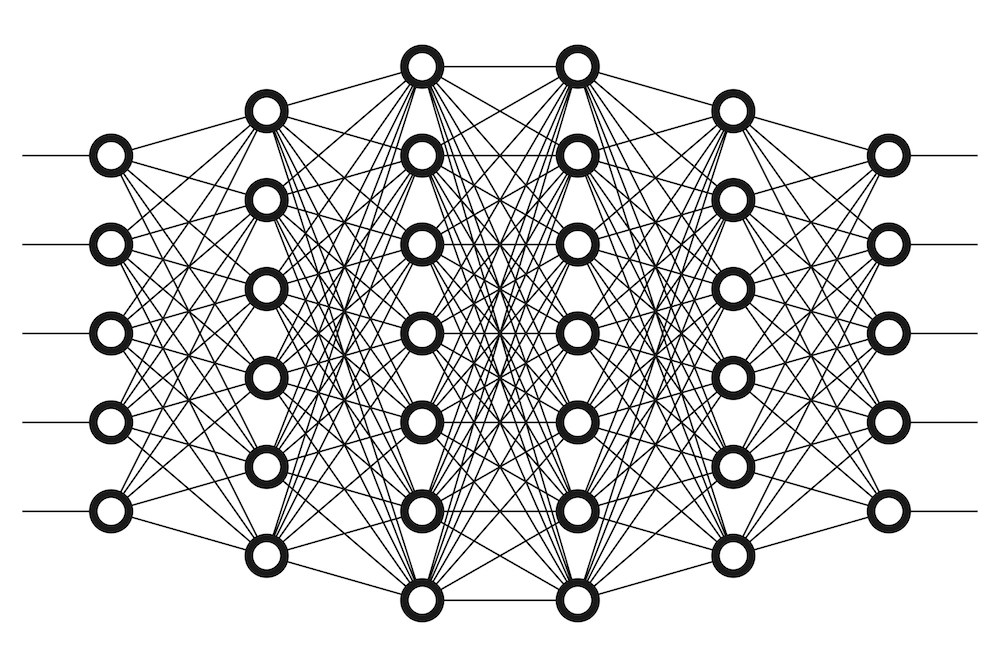
\includegraphics[width=\linewidth]{images/DeepNeuralNetwork.jpg}
  		\caption{Topologie eines \gls{FCNN}.\cite{NeuronalesNetzImage} }
  		\label{fig:Neuronales Netz}
\end{figure}

Diese Netze sind Programmiergerüste (\textit{Engl: Frameworks}) für Algorithmen, die auf maschinellem Lernen basieren. Beschrieben werden sie mit Begriffen aus der Biologie. Ein  \gls{ANN}, besteht aus einer gewissen Anzahl an Knoten, sogenannten \textit{Neuronen}, die bei unterschiedlichen Eingaben unterschiedlich aktiviert werden. Diese sind mit weiteren Neuronen über sogenannte \textit{Synapsen} verbunden und versenden je nach \gls{ANN}s mehr oder weniger starke Signale über diese Verbindungen.
Wie in Abbildung 2.1 dargestellt, können Neuronen in Lagen (\textit{Layers}) zusammengefasst werden, welche die Stufen des \gls{ANN}s darstellen, die mithilfe der Breitensuche bestimmt werden können.
Die erste Lage wird als \textit{inputlayer} beschrieben und die letzte Lage wird \textit{outputlayer} genannt. Jede Lage zwischen diesen beiden werden als \textit{hidden layers} beschrieben, weil sie nicht mit der Systemumgebung kommunizieren.\newline
Wie in unserem Beispiel erwähnt, ist das Ziel von neuronalen Netzen Eigenschaften zu erkennen, die gewisse Objekte gemeinsam haben. \gls{ANN}s sollen:
\begin{itemize}
	\item Klassifizieren
	\item Zusammenhänge erkennen
\end{itemize}

Es folgt nun eine kurze Beschreibung einiger ausgewählter Bestandteile von \gls{ANN}s, um über deren Funktionsweise einen Überblick zu bekommen.
\section{Aktivierungsfunktion}
Informationen werden in \gls{ANN} über Signale von Neuron zu Neuron weitergegeben. Jedoch werden diese Signale nicht direkt weitergegeben sonder müssen umgewandelt werden. Das Ausgabesignal eines Neurons wird durch die Aktivierungsfunktion berechnet. Diese bildet den Aktivierungswert auf ein Intervall ab und ist daher eine nichtlineare Funktion. Ohne diese Nichtlinearität könnten komplexe Datensätze wie Bilder, Videos sowie Audio nicht analysiert werden. Prägnant wird dies durch folgendes Zitat beschrieben:
\clearpage
\textit{''Neural-Networks are considered Universal Function Approximators. It means that they can compute and learn any function at all. Almost any process we can think of can be represented as a functional computation in Neural Networks.'' \cite{walia_2017}} Dies bedeutet, das \gls{ANN} sehr vielfältig angewendet werden können. Eine früher beliebte Aktivierungsfunktion war die \textit{normalisierte Sigmoid Funktion}.
\begin{equation} 
f(x) = \frac{1}{1 + e^{-x}},\ x\ die\ Eingabe,\ f(x)\ die\ Ausgabe\ des\ Neurones.
\end{equation}
%$}, mit x die Eingabe, f(x) die Ausgabe des Neurones.$
Während dies die wohl allgemein bekannteste Aktivierungsfunktion ist, verwenden moderne \gls{ANN}s heute eine Variante der \textit{Rectifier Funktion}, welche sich besser eignet zum trainieren von \gls{ANN}s \cite{lecun_bengio_hinton_2015}
\begin{equation}
g(x) = max(0, x),\ x\ die\ Eingabe,\ g(x)\ die\ Ausgabe\ des\ Neurones.
\end{equation}
Eine beliebte Approximation dieser Funktion ist z.B. die analytische Funktion
\begin{equation}
h(x) = log(1 + e^{x}),\ x\ die\ Eingabe,\ h(x)\ die\ Ausgabe\ des\ Neurones.
\end{equation}

\section{Propagierungsfunktion}

Jede Verbindung zwischen zwei Neuronen besitzt eine Gewichtung (\textit{Engl: weight}). Diese beschreibt wie viel Einfluss sie auf die Aktivierung des verbundenen Neurons ausübt.

Die \textit{Propagierungsfunktion} berechnet den Input $p_j^{l}(t)$ des Neurons j anhand der Outputs $o_i(t)$ der Neuronen in der vorangehenden Lage $l$.
\begin{align*}
p_j^{(l+1)}(t) &= \sum_{i}^{} o_i^{(l)}(t) w_{ij}^{(l)}
\end{align*}
Um eine Aktivierungsschwelle (\textit{Engl: threshold}) einzuführen, kann ein sogenannter \textit{bias} der Summe hinzugefügt werden. Dies ist nötig, wenn ein Neuron nur ab einem bestimmten Aktivierungswert von Bedeutung ist.
\begin{align*}
p_j^{(l+1)}(t) &= \sum_{i}^{} o_i^{(l)}(t) w_{ij}^{(l)} - bias
\end{align*}
Ein großer Vorteil von \gls{ANN}s ist, dass sie als eine Folge von Matrixmultiplikationen und Anwendung der Aktivierungsfunktion darstellbar sind, welche besonders effizient durch Computerprozessoren berechnet werden können.
\begin{center}
\begin{figure}[H]
		\center
  		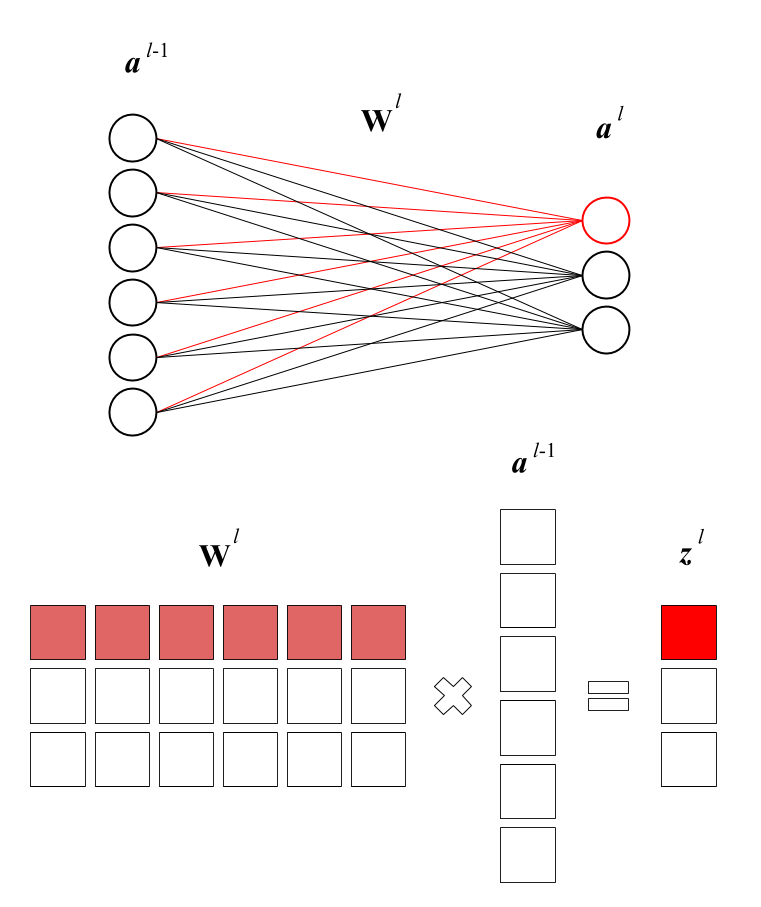
\includegraphics[scale=0.3]{images/NNMatrix.png}
  		\caption{Neuronales Netz in Matrixdarstellung. Hierbei ist $a^{l} = f(z^{l})$ wobei $f$ die Aktivierungsfunktion darstellt. \cite{hallstroem_2016}}
  		\label{fig:Neuronales Netz in Matrixdarstellung}
\end{figure}
\end{center}

%\subsection{Fully Connected Layers}
%\subsection{Convolution}
%\subsection{Pooling}
%\subsection{Reccurence}
\section{Trainieren eines \gls{ANN}}
Wie zuvor beschrieben, benötigt ein \gls{ANN} massive Datensätze. Zum Trainieren wird ein Algorithmus genutzt, der anhand dieser Daten die \textit{weights} und \textit{biases} so einstellt, dass das Netzwerk seine Funktion erfüllt. Dies ist wegen der massiven Anzahl an Parametern (Größenordnungen von $10^{6}$ Parametern werden bei modernen Netzen erreicht \cite{szegedy2015going}) nichttrivial. Ein weitverbreiteter Algorithmus ist die Fehlerrückführung (\textit{Backpropagation}).

\section{Backpropagation}
Der Backpropagation Algorithmus verläuft folgendermaßen \cite{BibEntry2019Jan}: erst werden Eingabemuster durch das \gls{ANN} propagiert, daraufhin wird die Ausgabe des Netzes, d.h. die Aktivierung des letzten Layers verglichen mit der gewünschten Aktivierung und der Fehler des Netzes durch die Summe der Quadrate der Abweichungen berechnet.
\begin{align*}
E &= \dfrac{1}{2}{\sum_{i=1}^{n}(t_i - o_i)^2},\ mit
\end{align*}
\textit{$E$ die Fehlerfunktion} \\
\textit{$t_i$ der gewünschte Output beim Muster i} \\
\textit{$o_i$ der wirkliche Output beim Muster i} \\
\textit{$n$ die Anzahl an Mustern, die dem Netz vorgestellt werden}

Das Ziel ist es nun die Summe der Fehlerfunktionen über alle möglichen Inputs zu minimieren. Dies ist nicht möglich ohne alle möglichen Kombinationen von \textit{weights} (und falls vorhanden \textit{biases}) auszuprobieren, jedoch ist es möglich dank des Gradientenverfahrens lokalen Minimas nahe kommen.


\section{Fehlerminimierung}
Sei $w_{ij}$ das Gewicht der Verbindung des Neurones $i$ zum Neuron $j$. Wir versuchen dieses nun so anzupassen, das die Fehlerfunktion minimiert wird. Dazu muss die partielle Ableitung der Fehlerfunktion $E$ berechnet werden:
\begin{equation}
\frac{\partial E}{\partial w_{ij}}
\end{equation}
mit einem Lernfaktor $\eta$ kann eingestellt werden, wie schnell das Neuronale Netz sich dem Lokalen Minimum nähert. Jedoch können zu starke Korrekturen \textit{\grqq{}über das Ziel hinausschießen\grqq{}} d.h. einem lokalen Minimum außer durch Zufall nicht nahe genug kommen und somit den Nutzen des Trainierens beschränken. Wir definieren infolgedessen die Änderung des Gewichtes $\Delta w_{ij}$ als:
\begin{equation}
\Delta w_{ij} = -\eta \frac{\partial E}{\partial w_{ij}}
\end{equation}
Und somit können wir die Änderung der Gewichte folglich vornehmen:
\begin{equation}
w_{ij}^{neu} = w_{ij}^{alt} + \Delta w_{ij},\ mit
\end{equation}
\textit{$w_{ij}^{neu}$ der neue Wert des Gewichts der Verbindung zwischen Neuronen i und j\\
$w_{ij}^{alt}$ der alte Wert des Gewichts	der Verbindung zwischen Neuronen i und j	\\
$\Delta w_{ij}$ die Änderung des Gewichts der Verbindung zwischen Neuronen i und j}

\section{Limitationen und Gefahren von Neuronalen Netzen}
Während sich \gls{ANN}s im Moment großer Beliebtheit erfreuen, ist es wichtig einiger ihrer Nachteile bewusst zu sein. Wie zuvor erwähnt, werden durch das Gradientenverfahren nur lokale Minima gefunden. Die Performance eines \gls{ANN} nach dem Trainieren ist daher stark von den Anfangswerten der weights und biases abhängig und kann unter Umständen auf enttäuschendem Niveau stagnieren, unabhängig davon wie viele Daten zur Verfügung stehen. Das Trainieren von \gls{ANN}s ist noch immer sehr Rechnerleistungsintensiv und benötigt große Mengen an vorklassifizierten Daten (\text{labeled data}), die nicht immer zur Verfügung stehen.  Durch diese neuen Technologien sind Daten sehr wertvoll geworden. Während \gls{MaschinellesLernen} zwar nicht verantwortlich ist für den unvorsichtigen Umgang und Handel mit unseren Daten, so verstärken sie diesen Trend. Es wird oft angenommen, das es nicht möglich sei ein \gls{ANN} zu verstehen, da es sich um eine \textit{black box} handele. Obwohl einige Fortschritte im Verständnis der inneren Funktion von trainierten \gls{ANN}s gemacht worden sind \cite{lime}, ist es noch immer schwierig trainierte \gls{ANN}s oder ähnliche Konstrukte zu verstehen. Es sollte immer damit gerechnet werden, dass ein neuronales Netz auf völlig vorhergesehene Weise auf eine neue Eingabe reagiert. Es können kaum Garantien für das Verhalten eines neuronalen Netzes gegeben werden. Anwendungen von \gls{ANN}s und der damit verbundene Kontrollverlust werfen ethische Fragen auf, mit denen wir uns auseinandersetzen müssen \cite{gibbs_2018}.

Trotz dieser Bedenken hat Maschinelles Lernen große Fortschritte in vielen Bereichen der Informatik ermöglicht. Im Bereich der Programmierung in Natürlicher Sprache basiert ein großer Teil der Anwendungssoftware auf Maschinellem Lernen. Ein Beispiel dieser Anwendungssoftware ist sind automatische Übersetzungen, welche heutzutage auf \gls{ANN}s basieren.

\let\cleardoublepage\relax \chapter{Maschinelle Übersetzungen (\gls{MT})}

\section{Neuronale Maschinenübersetzung (\gls{NMT})}

 Während Chatbots noch weit davon entfernt sind den \gls{Turingtest} zu bestehen, so haben Maschinelle Übersetzungen dank \gls{ANN}s quasi menschliche Fehlerraten erreicht \cite{googleaiblog_2016}.
 
\begin{figure}[H]
  \center
  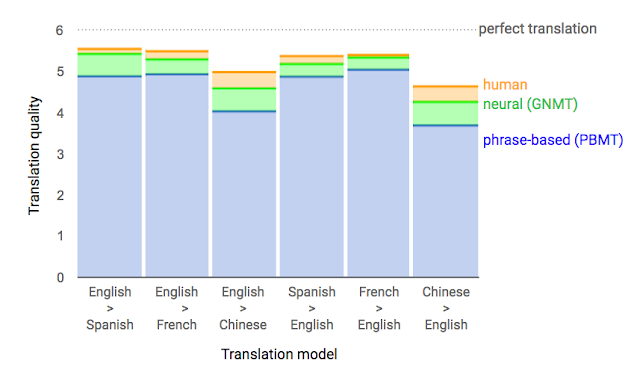
\includegraphics[width=\textwidth]{images/MTGoogle.png}
  \caption{Personen mit exzellenten Sprachkenntnissen in der Ursprungs und Zielsprache wurden gebeten Übersetzungen von Google Translate auf einer Skala von 0 bis 6 zu bewerten. \cite{googleaiblog_2016}}
  \label{fig:GoogleTranslate Performance}
\end{figure}

Wie in Abbildung 3.1 zu erkennen ist, hat \gls{NMT} signifikative Verbesserungen in \gls{MT} ermöglicht. Dank \gls{ANN}s behauptet Google z.B. ihre Fehlerraten um 60\% gesenkt zu haben \cite{wu2016google}. Andere Dienste wie Microsoft sowie Yahoo melden ähnliche Fortschritte \cite{Microsoft2018}.

\section{Long short-term memory}
Moderne neurale Übersetzungsmaschinen (\gls{NMT}) nutzen Long short-term memory Netze  \cite{DBLP:journals/corr/WuSCLNMKCGMKSJL16}. Eine Form dieser Netzwerke sind die Rekursiven Neuronale Netzen. Diese \gls{ANN}s haben die Eigenschaft, dass sie zyklische Verbindungen erlauben und somit sequentielle Eingaben verarbeiten können. Diese gelten als besonders schwierig zu implementieren sind aber essentiell zur Analyse von Daten wie gesprochener oder geschriebener Text. Betrachten wir als Beispiel das Elman Netzwerk:
\begin{figure}[H]
		\center
  		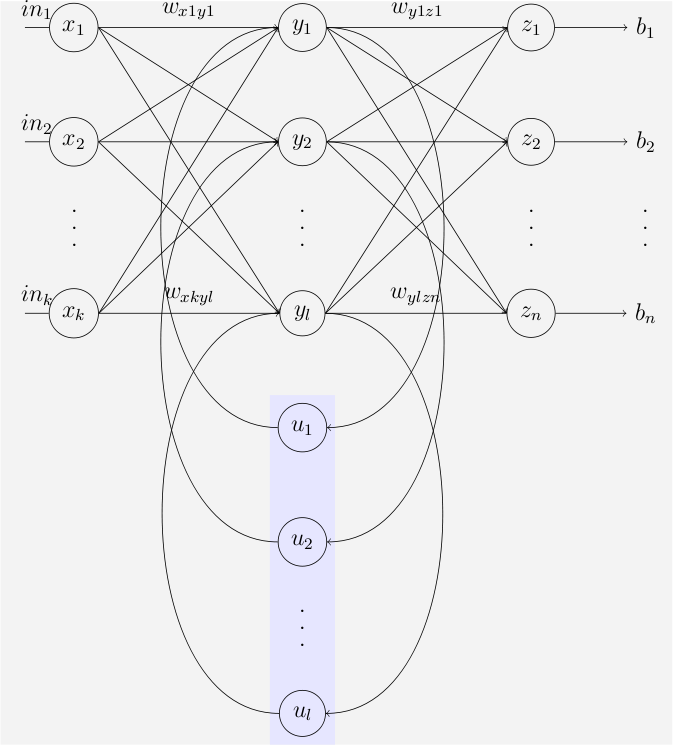
\includegraphics[scale=0.55]{images/Elman_RNN.png}
  		\caption{Das Elman Netzwerk\cite{Elman}}
  		\label{fig:Elman Netzwerk}
\end{figure}
In Abbildung 3.2 sind Rückwärtsverbindungen dargestellt. Es gibt einerseits eine Vorwärtsverbindung von $y_l$ nach $u_l$ sowie eine Rückwärtsverbindung von $u_l$ nach $y_l$.  Die Rückwärtsverbindungen merken sich eine Kopie des Aktivierungsgraded ihres Ausgangsneurons. Dadurch können Eingaben gespeichert werden und bei neuen Eingaben in Betracht gezogen werden. Dadurch wird sequentielle Betrachtung von Daten ermöglicht.
In der Praxis werden weitaus komplexere neuronale Netze verwendet  \cite{dellaert1996recognizing}, welche aber auf denselben Mechanismen basieren wie die hier beschriebenen. Nennenswert sind z.B. Convolutional Neural Networks, das Hopfield Netzwerk, die Boltzmann Maschine, sowie Autoencoders. Diese im Detail zu beschreiben würde jedoch den Rahmen dieser Arbeit sprengen.
%\begin{itemize}
	%\item Recurrent Neural Networks
		%[Warum gerade diese?]
		%[Elman Network, Jordan Netzwerk, Hopfield Network,...]
	%\item 
%\end{itemize}

%\section{Kuriositäten}

%Algorithmen die auf \gls{MaschinellesLernen} und insbesondere auf \gls{ANN} basieren sind oft unvorhersehbar und finden manchmal bemerkenswerte Lösungswege.
%\begin{itemize}
	%\item Facebook Chatbots haben eine eigene Sprache erfunden um zu kommunizieren\cite{wilson_2018}.
%	\item Google Translate hat eine Sprache erfunden die als Zwischensprache dient \cite{googleAiblog_2016Translation}.
%\end{itemize}
%Facebook hat zwei Chatbots verschiedene virtuelle Objekte gegeben, welche einen bestimmten Wert besaßen. Die Bots sollten Tauschhandel betreiben. Die Verhandlungstaktiken, die die beiden Chatbots nutzen, sollten durch \gls{MaschinellesLernen} erlernt werden.

%\begin{figure}[H]
  %\center
  %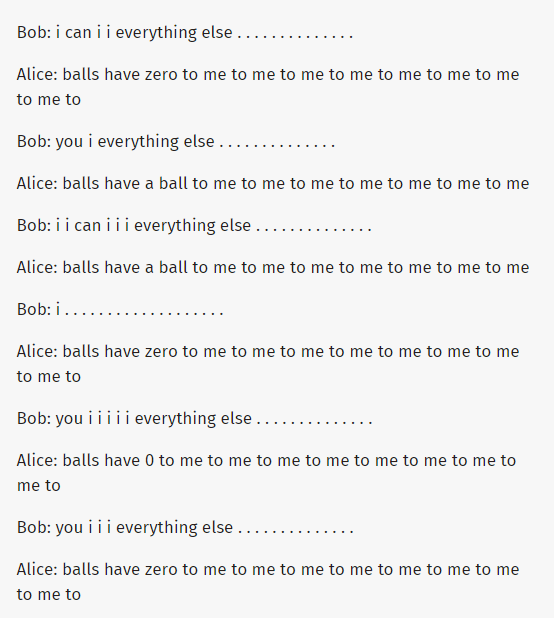
\includegraphics[scale=0.6]{images/FacebookChatbots.png}
  %\caption{Facebook Chatbots entwickeln ihre eigene Sprache. \cite{wilson_2018}}
  %\label{fig:Facebook Chatbots}
%\end{figure}

%Dass die Chatbots beschließen nicht mehr auf Englisch zu Kommunizieren hatte niemand vorausgesehen. Es zeigt auf wie unvorhergesehen sich \gls{MaschinellesLernen} Algorithmen verhalten können.
%\newline
%\newline
%Bevor Google translate \gls{ANN} verwendete, wurde jeder Satz erst ins Englische und dann in die Zielsprache übersetzt. Diese Methode limitiert die Anzahl an Übersetzungen die Programmiert werden müssen drastisch, schlägt jedoch fehl sobald das Wort das übersetzt werden muss nicht im englischen vorkommt. Das \gls{ANN} das von Google seit kurzem eingesetzt wird hat eine neue Sprache entwickelt. Jeder Satz wird nun erst in die entwickelte Sprache übersetzt und dann in die Zielsprache. In dieser Sprache gibt es z.B ein Wort für Baum. Dieses ist verlinkt mit jedem Wort in jeder Sprache, das Baum bedeutet. Man bemerkt das das neuronale Netz denselben Ansatz verwendet hat, den Menschen zuvor auch angewandt haben, jedoch ein Schritt weiter gegangen ist.

\chapter{Bewertung} 
\gls{MaschinellesLernen} ist ein mächtiges Werkzeug in vielen Bereichen der Informatik. Insbesondere \gls{ANN}s haben Teile der Informatik schon revolutioniert.
Jedoch besitzen diese Werkzeuge, dieselben Probleme die wir Menschen auch haben. Sie sind nur so gut wie die Daten, die ihnen zum Trainieren zur Verfügung gestellt werden. Des Weiteren sind genaue Lösungswege nur schwer zu durchschauen. Sprachen verändern sich ständig, daher ist es von nutzen, das Übersetzungstools ebenso dem allgemeinen Sprachgebrauch anpassen.

%% --------------------
%% |   Bibliography   |
%% --------------------
\cleardoublepage
\phantomsection
\addcontentsline{toc}{chapter}{\bibname}

\iflanguage{english}
{\bibliographystyle{IEEEtranSA}}	% english style with numeric references
{\bibliographystyle{alphadin}}	% german style

\bibliography{thesis}


%% ----------------
%% |   Appendix   |
%% ----------------
%\cleardoublepage
%%% appendix.tex
%%

%% ==============================
%\chapter{Appendix}
%\label{ch:Appendix}
%% ==============================

\appendix

\iflanguage{english}
{\addchap{Appendix}}	% english style
{\addchap{Anhang}}	% german style


...



%% ----------------
%% |   Glossary   |
%% ----------------
\cleardoublepage
\printglossary

\end{document}
